\documentclass[11pt,a4paper]{article}
\usepackage[utf8]{inputenc}
\usepackage[T1]{fontenc}
\usepackage[french]{babel}
\usepackage{amsmath,amssymb}
\usepackage{geometry}
\usepackage{fancyhdr}
\usepackage{enumitem}
\usepackage{multicol}
\usepackage{tikz}
\usepackage{pgfplots}
\pgfplotsset{compat=1.18}  % Ajout pour éviter l'avertissement
\usepackage{xcolor}
\usepackage{graphicx}
\usepackage{array}
\usepackage{fontawesome5}
\usepackage{tabularx}
\usepackage[most]{tcolorbox}  % Un seul appel au package

% Définition des couleurs modernes
\definecolor{primary}{RGB}{41, 128, 185}      % Bleu moderne
\definecolor{secondary}{RGB}{52, 73, 94}      % Gris foncé
\definecolor{accent}{RGB}{46, 204, 113}       % Vert menthe
\definecolor{warning}{RGB}{231, 76, 60}       % Rouge moderne
\definecolor{light}{RGB}{236, 240, 241}       % Gris très clair
\definecolor{bglight}{RGB}{247, 249, 250}     % Fond clair

\DeclareRobustCommand{\rep}[1]{\begingroup\color{warning}\ifmmode #1\else \textbf{#1}\fi\endgroup}

% Configuration de la page
\geometry{
	top=1.5cm,
	bottom=2cm,
	left=1.8cm,
	right=1.8cm
}

% Configuration tcolorbox
\tcbuselibrary{skins,breakable}

% Boîte pour les exercices
\newtcolorbox{exercisebox}[2][]{
	colback=white,
	colframe=primary,
	fonttitle=\bfseries\large,
	title={#2},
	arc=2mm,
	boxrule=1.5pt,
	left=15pt,
	right=15pt,
	top=12pt,
	bottom=12pt,
	boxsep=0pt,
	breakable,
	enhanced,
	width=\linewidth,
	grow to left by=3mm,
	grow to right by=3mm,
	#1
}

% Boîte pour les consignes
\newtcolorbox{consignebox}{
	colback=light!30,
	colframe=secondary,
	arc=3mm,
	boxrule=0pt,
	leftrule=4pt,
	left=15pt,
	right=15pt,
	top=12pt,
	bottom=12pt,
	enhanced,
	width=\linewidth,
	grow to left by=3mm,
	grow to right by=3mm
}

% Boîte pour les compétences
\newtcolorbox{competencebox}{
	colback=accent!10,
	colframe=accent,
	arc=2mm,
	boxrule=0.5pt,
	left=10pt,
	right=10pt,
	top=8pt,
	bottom=8pt,
	fontupper=\small\itshape,
	enhanced,
	width=\linewidth
}

% En-tête et pied de page personnalisés
\pagestyle{fancy}
\fancyhf{}
\fancyhead[L]{\color{secondary}\textbf{4\textsuperscript{e}} | Mathématiques}
\fancyhead[R]{\color{secondary}\textbf{Nombres Relatifs}}
\fancyfoot[C]{\color{secondary}\thepage}
\renewcommand{\headrulewidth}{0pt}
\renewcommand{\footrulewidth}{0pt}

% Commandes personnalisées
\newcommand{\points}[1]{\hfill \colorbox{primary}{\color{white}\textbf{\,#1 pts\,}}}
\newcommand{\badge}[2]{\tikz[baseline=(char.base)]{\node[shape=rectangle,draw,thick,rounded corners=2mm,inner sep=2pt,fill=#1,text=white,font=\footnotesize\bfseries] (char) {#2};}}

% Pointillés de longueur fixe, rendu de \dotfill
\newcommand{\dotline}[1]{\makebox[#1][s]{\dotfill}}

\newcolumntype{L}[1]{>{\hsize=#1\hsize\arraybackslash}X} % X pondéré

% Nouvelle commande pour les zones de réponse
\newcommand{\zonereponse}[1]{%
	\par\noindent
	\colorbox{light}{%
		\parbox{\dimexpr\linewidth-2\fboxsep\relax}{%
			\vspace{#1}%
		}%
	}%
	\par
}

% Lignes en pointillés — par nombre de lignes
\newcommand{\zonereponseLignes}[2][0.9cm]{%
	\par\noindent
	\colorbox{light}{%
		\parbox{\dimexpr\linewidth-2\fboxsep\relax}{%
			\setlength{\parskip}{#1}%
			\foreach \i in {1,...,#2}{\noindent\dotfill\par}%
		}%
	}\par
}

% Lignes en pointillés — par hauteur totale
\newcommand{\zonereponseHauteur}[2][0.9cm]{%
	\par\noindent
	\colorbox{light}{%
		\parbox{\dimexpr\linewidth-2\fboxsep\relax}{%
			\leaders\vbox to #1{\vfil\hbox to \hsize{\dotfill}\vfil}\vskip #2\relax
		}%
	}\par
}

\begin{document}
	
	% En-tête moderne avec TikZ
	\begin{tikzpicture}[remember picture,overlay]
		\fill[primary] (current page.north west) rectangle ([yshift=-3.5cm]current page.north east);
		\node[anchor=north west,text=white,font=\Huge\bfseries] at ([xshift=2cm,yshift=-1cm]current page.north west) {Contrôle \no 1};
		\node[anchor=north west,text=white,font=\Large] at ([xshift=2cm,yshift=-2cm]current page.north west) {Nombres Relatifs \& Enchaînement d'Opérations};
		\node[anchor=north east,text=white,font=\large] at ([xshift=-2cm,yshift=-1.5cm]current page.north east) {\faIcon{clock} 55 minutes};
		\node[anchor=north east,text=white,font=\large] at ([xshift=-2cm,yshift=-2.3cm]current page.north east) {\faIcon{calculator} Calculatrice interdite};
	\end{tikzpicture}
	
	\vspace{2cm}
	
	% Informations élève dans un tableau moderne
	\begin{tcolorbox}[
		colback=bglight,colframe=secondary,arc=3mm,boxrule=1pt,
		left=15pt,right=15pt,top=10pt,bottom=10pt,
		enhanced,
		width=\linewidth,
		grow to left by=5mm,
		grow to right by=5mm
		]
		\setlength{\tabcolsep}{4pt} % espace intercolonnes
		\begin{tabularx}{\linewidth}{@{}lX lX l@{}}
			% Ligne 1 : 2 colonnes (NOM, Prénom)
			\multicolumn{2}{@{}l}{\faIcon{user} \textbf{NOM :} \dotline{6cm}} &
			\multicolumn{2}{l@{}}{\textbf{Prénom :} \dotline{3cm}} &
			\\[0.5cm]
			% Ligne 2 : 3 colonnes (Classe, Date, Note)
			\textbf{Classe :} & \dotfill &
			\faIcon{calendar} \textbf{Date :} & \dotfill &
			\fcolorbox{secondary}{white}{\textbf{NOTE : }\makebox[1.4cm]{\rule{0pt}{1.1em}}\textbf{ / 20}}
		\end{tabularx}
	\end{tcolorbox}
	
	\vspace{0.3cm}
	
	% Barème et compétences
	\begin{center}
		\badge{primary}{Ex.1: 4pts} \quad
		\badge{primary}{Ex.2: 4pts} \quad
		\badge{primary}{Ex.3: 8pts} \quad
		\badge{primary}{Ex.4: 4pts} \quad
		\badge{accent}{Bonus: +2pts}
	\end{center}
	
	\vspace{0.3cm}
	
	% Consignes
	\begin{consignebox}
		\faIcon{info-circle} \textbf{CONSIGNES IMPORTANTES}
		\begin{itemize}[leftmargin=*,noitemsep,topsep=5pt]
			\item[\faIcon{check}] Rédigez clairement et justifiez tous vos calculs
			\item[\faIcon{check}] Respectez les priorités opératoires
			\item[\faIcon{check}] Les exercices peuvent être traités dans n'importe quel ordre
			\item[\faIcon{times}] Calculatrice non autorisée
		\end{itemize}
	\end{consignebox}
	
	\vspace{0.5cm}
	\begin{exercisebox}{\faIcon{list-ul} QCM : Nombres relatifs \points{4}}
		Pour chaque question, écris la lettre de la seule réponse correcte dans la colonne de droite :
		\begin{center}
			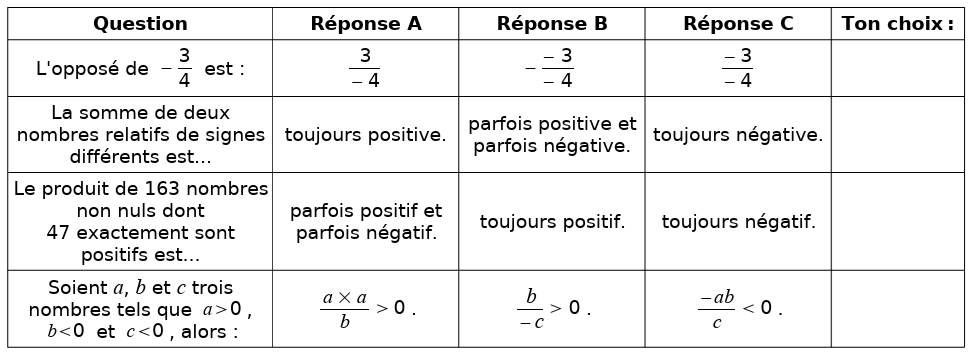
\includegraphics[width=1\linewidth]{images/qcm}
		\end{center}
		
	\end{exercisebox}
	
	% Exercice 1
	\begin{exercisebox}{\faIcon{edit} Exercice 1 : Opérations de base \points{4}}
		
		\vspace{0.2cm}
		\textbf{Calculer les expressions suivantes :}
		
		\begin{multicols}{2}
			\begin{enumerate}[label=\textcolor{primary}{\textbf{\alph*)}},leftmargin=*]
				\item $(-8) + (+5) = $ \dotfill \points{1}
				\vspace{0.8cm}
				
				\item $(-3) - (-7) = $ \dotfill \points{1}
				\vspace{0.8cm}
				
				\item $(+6) \times (-4) = $ \dotfill \points{1}
				\vspace{0.8cm}
				
				\item $(-36) \div (+9) = $ \dotfill \points{1}
			\end{enumerate}
		\end{multicols}
	\end{exercisebox}
	
	% Exercice 2
	\begin{exercisebox}{\faIcon{layer-group} Exercice 2 : Priorités opératoires \points{8}}
		%		\begin{competencebox}
			%			\faIcon{bullseye} Compétence : Respecter l'ordre des opérations dans un calcul
			%		\end{competencebox}
		
		\vspace{0.3cm}
		\textbf{Calculer en détaillant toutes les étapes :}
		
		\begin{enumerate}[label=\textcolor{primary}{\textbf{\alph*)}},leftmargin=*]
			\item $A = -4 + 6 \times (-3)$ \points{1}
			
			\zonereponseLignes[0.50cm]{4}
			
			\item $B = 18 - 2 \times (5 - 9)$ \points{1}
			
			\zonereponseLignes[0.50cm]{4}
			
			\item $C = \dfrac{-15 + 3}{-4} - 7$ \points{2}
			
			\zonereponseLignes[0.50cm]{4}
			
			\item $D = 3 \times [(-4) + 7] - 2 \times (-6 + 3)$ \points{2}
			
			\zonereponseLignes[0.40cm]{7}
			
			\item $E = \dfrac{(-2)^2 + 4 \times 3}{-5 + 2}$ \points{2}
			\zonereponseLignes[0.50cm]{4}
		\end{enumerate}
	\end{exercisebox}
	
	%\newpage
	
	
	
	
	% Exercice 3
	\begin{exercisebox}{\faIcon{lightbulb} Exercice 3 : Résolution de problème \points{4}}
		%		\begin{competencebox}
			%			\faIcon{bullseye} Compétence : Modéliser une situation et résoudre un problème
			%		\end{competencebox}
		
		\vspace{0.01cm}
		
		\begin{tcolorbox}[colback=blue!5,colframe=primary!30,arc=2mm,boxrule=0.5pt]
			\textbf{Contexte :} Un sous-marin se trouve à une profondeur de $-120$ mètres. 
			\begin{itemize}[noitemsep,topsep=5pt]
				\item Il remonte d'abord de 45 mètres
				\item Puis il descend de 30 mètres
				\item Enfin, il remonte de 25 mètres
			\end{itemize}
		\end{tcolorbox}
		
		\begin{enumerate}[leftmargin=*]
			\item \textbf{Écrire l'expression mathématique} qui permet de calculer la profondeur finale : \points{1.5}
			
			\zonereponseLignes[0.40cm]{3}
			
			\item \textbf{Calculer} cette profondeur finale : \points{1.5}
			
			\zonereponseLignes[0.40cm]{4}
			
			\item \textbf{Question :} Le sous-marin veut atteindre $-50$ mètres. Doit-il monter ou descendre ? De combien de mètres ? \points{1}
			
			\zonereponseLignes[0.40cm]{3}
		\end{enumerate}
	\end{exercisebox}
	
	\vspace{0.2cm}
	
	% Bonus
	\begin{tcolorbox}[
		colback=accent!10,
		colframe=accent,
		fonttitle=\bfseries,
		title={\faIcon{star} BONUS : Défi \badge{accent}{+2pts}},
		arc=3mm,
		boxrule=1.5pt,
		enhanced,
		width=\linewidth,
		grow to left by=3mm,
		grow to right by=3mm
		]
		Soit l'expression : $G = \dfrac{2a - b^2}{c + d}$
		
		Avec : $a = -4$ ; $b = -3$ ; $c = -5$ ; $d = 2$
		
		Calculer $G$ en remplaçant et en détaillant toutes les étapes.
		\zonereponseLignes[0.40cm]{7}
	\end{tcolorbox}
	
	% Pied de page avec évaluation
	\vspace{0.2cm}
	\begin{center}
		\begin{tikzpicture}
			\node[draw=secondary,rounded corners=3mm,inner sep=8pt,fill=light!30] {
				\begin{tabular}{lccccc}
					\textbf{Auto-évaluation :} & 
					\faIcon{frown} Difficile & 
					\faIcon{meh} Moyen & 
					\faIcon{smile} Facile & 
					\phantom{xx} & 
					\textbf{Temps utilisé :} \underline{\phantom{xxxxx}} min
				\end{tabular}
			};
		\end{tikzpicture}
	\end{center}
	
	\newpage
	% =======================
	% CORRIGÉ
	% =======================
	
	\begin{exercisebox}{\faIcon{list-ul} QCM : Nombres relatifs — Corrigé}
		Pour chaque question, réponse correcte en \rep{rouge}.
		
		L'opposé de $-\dfrac{3}{4}$ est \rep{$\dfrac{3}{4} = \dfrac{-3}{-4}$}.
		La somme de deux nombres relatifs de signes différents est \rep{parfois positive et parfois négative}.
		Le produit de 163 nombres non nuls dont 47 sont positifs est \rep{toujours positif} (il reste 116 négatifs, nombre pair).
		Soient $a>0$, $b<0$, $c<0$. Vrai: \rep{$\dfrac{-ab}{c}<0$} (car $ab<0\Rightarrow -ab>0$ et $c<0$, donc quotient négatif).
	\end{exercisebox}
	\begin{exercisebox}{\faIcon{edit} Exercice 1 — Corrigé}
		a) $(-8)+(+5)=\rep{-3}$
		
		b) $(-3)-(-7)=-3+7=\rep{4}$
		
		c) $(+6)\times(-4)=\rep{-24}$
		
		d) $(-36)\div(+9)=\rep{-4}$
	\end{exercisebox}
	
	\begin{exercisebox}{\faIcon{layer-group} Exercice 2 — Corrigé}
		a) $A=-4+6\times(-3)=-4-18=\rep{-22}$
		
		b) $B=18-2\times(5-9)=18-2\times(-4)=18-(-8)=\rep{26}$
		
		c) $C=\dfrac{-15+3}{-4}-7=\dfrac{-12}{-4}-7=3-7=\rep{-4}$
		
		d) $D=3\times[(-4)+7]-2\times(-6+3)=3\times3-2\times(-3)=9-(-6)=\rep{15}$
		
		e) $E=\dfrac{(-2)^2+4\times3}{-5+2}=\dfrac{4+12}{-3}=\dfrac{16}{-3}=\rep{-\dfrac{16}{3}}$
	\end{exercisebox}
	
	\begin{exercisebox}{\faIcon{lightbulb} Exercice 3 — Corrigé}
		
		Expression: \quad \rep{-120+45-30+25}
		
		Calcul: \quad $-120+45=-75$, puis $-75-30=-105$, puis $-105+25=\rep{-80}$
		
		Vers $-50$ m: \quad de $-80$ à $-50$, il faut \rep{monter 30 m}.
	\end{exercisebox}
\end{document}